\chapter{Classification results evaluation} \label{chapt4}

\section{General steps} \label{sect4_1}
\noindent
In this section I need to:
\begin{itemize}
	\item visualize results of each training step, to understand hyperparameters better
	\item estimate networks by types 
	\item chose hyperparameters to gain the best evaluation metrics  
	\item train each network on different amount of epochs
	\item save network parameters and weights after each epoch. It will give me a possibility to restore the best model if network accuracy goes down.
\end{itemize}

\noindent
Training time is a very important parameter. Therefore, I would like to train NN models which have nearly the same training time. To make it easier to understand the results of NN, a famous suite of visualization tools called TensorBoard was used. With TensorBoard it is possible to visualize graphs, plot quantitative metrics and show additional data like images passing through it.  


\section{Base line model} \label{sect4_2}

Firstly, I built the baseline model which CNN models should achieve in the future. I started this step with LSTM networks, as most often mentioned in the articles on NLP problems. At this step I was trying different configurations of LSTM parameters. The architecture which gave me the best score is shown in the Figure \ref{img:part4-bilstm}. According to my experiments bidirectional recurrent networks perform better than the same type and same size by parameters one directional networks, therefore it was chosen as the main layer. As input to the NN I gave two embedded sequences of words: one for the description of advert , another for title. This model has the bi-LSTM layer with 100 units. Each sequence goes through the bi-LSTM layer and then merged together. To solve overfitting in this model I used BatchNormalization and dropout. LSTM dropout rate was chosen manually and was equal to 0.332. Besides the bi-LSTM layer, there are two fully connected layers: one at the end because we want to estimate probabilities for each class, so it has 183 neurons in it and one in the middle with 130 neurons. As a training algorithm I chose Adam with default parameters: (lr=0.001, beta\_1=0.9, beta\_2=0.999, epsilon=1e-08, decay=0.0). As I have mentioned earlier, to better understand the network I visualize the histograms and percentile weights in each layer. The model was trained on 15 epochs.


\begin{figure}[ht] 
	\center
	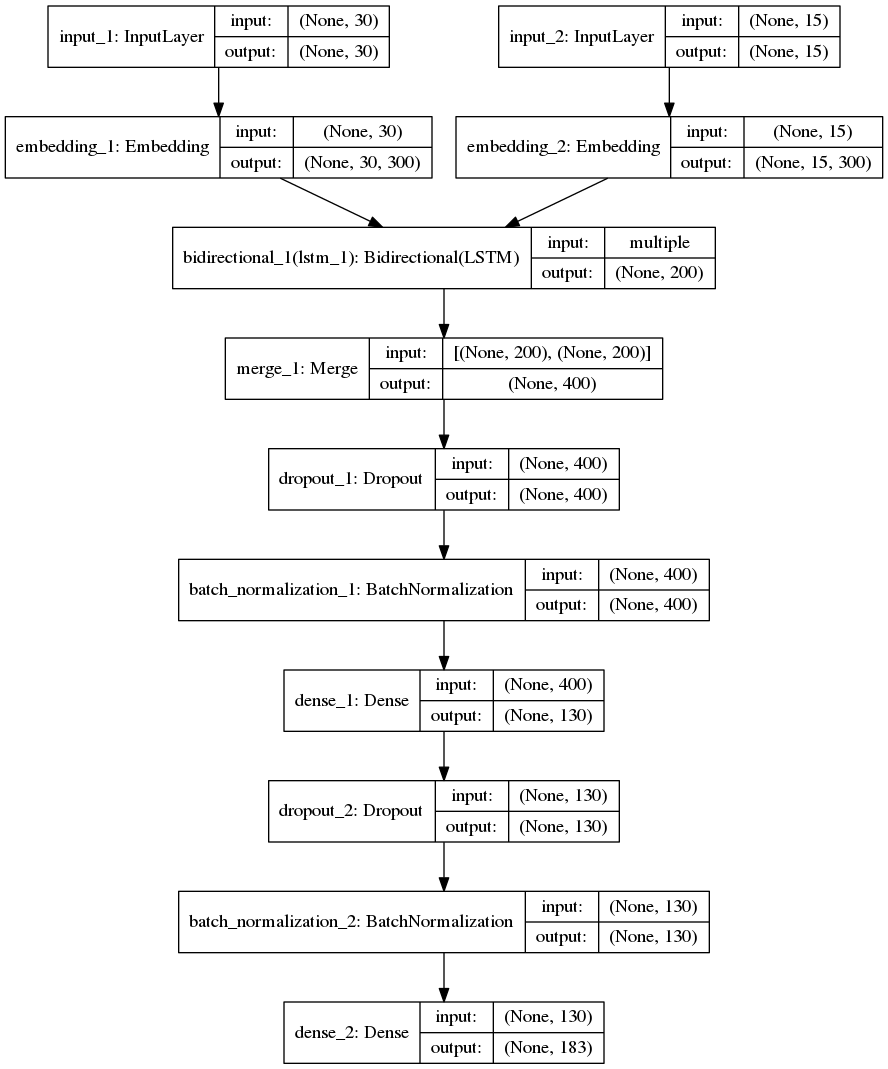
\includegraphics [scale=0.4] {part4/bilstm_architecture.png} 
	\caption{Architectures of Bi-LSTM models with 100 units } 
	\label{img:part4-bilstm} 
\end{figure}

As can be seen from the results of model training in Figure \ref{img:/bilstm_val_category_accuracy}, categorical accuracy on the training set and validation set performs equally well: 0.7975 and 0.8203 respectively. Surprisingly, the results on train are slightly better than on training data.   

\begin{figure}[ht]
	\begin{minipage}[ht]{1\linewidth}
		\center{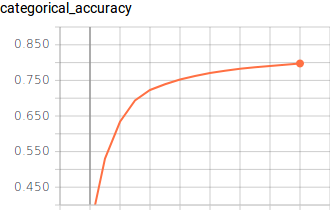
\includegraphics[width=0.5\linewidth]{part4/bilstm_train_category_accuracy}}
	\end{minipage}
	\hfill
	\begin{minipage}[ht]{1\linewidth}
		\center{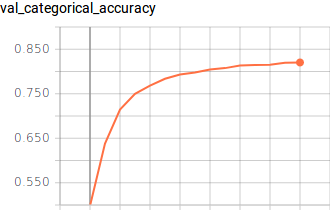
\includegraphics[width=0.5\linewidth]{part4/bilstm_val_category_accuracy}}
	\end{minipage}
	\caption{Models train and validation categorical accuracy by epochs}
	\label{img:/bilstm_val_category_accuracy}  
\end{figure}

Figure \ref{img:bilstm_val_category_crossentropy} shows that categorical cross entropy decrease on each epoch as it was expected. After 15 epochs results were the following: 0.8532 on the training set and 0.7478 on test.    

\begin{figure}[ht]
	\begin{minipage}[ht]{1\linewidth}
		\center{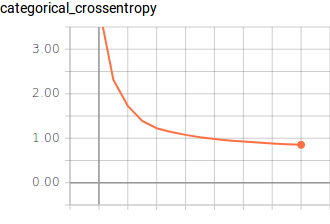
\includegraphics[width=0.5\linewidth]{part4/bilstm_train_category_crossentropy}}
	\end{minipage}
	\hfill
	\begin{minipage}[ht]{1\linewidth}
		\center{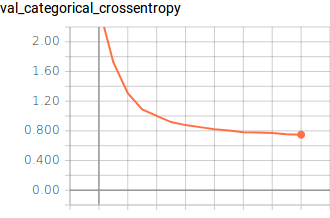
\includegraphics[width=0.5\linewidth]{part4/bilstm_val_category_crossentropy}}
	\end{minipage}
	\caption{Models train and validation category crossentropy by epochs}
	\label{img:bilstm_val_category_crossentropy}  
\end{figure}

The most important metric for this task was top categorical accuracy which can be seen in the Figure \ref{img:bilstm_val_top_k_accuracy}. On training data the model showed 0.9189 accuracy and on the test data - 0.9319.   

\begin{figure}[ht]
	\begin{minipage}[ht]{1\linewidth}
		\center{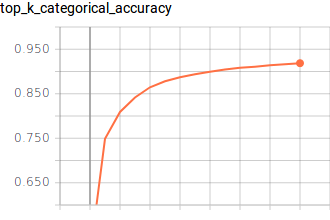
\includegraphics[width=0.5\linewidth]{part4/bilstm_train_top_k_accuracy}}
	\end{minipage}
	\hfill
	\begin{minipage}[ht]{1\linewidth}
		\center{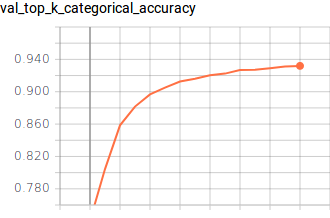
\includegraphics[width=0.5\linewidth]{part4/bilstm_val_top_k_accuracy}}
	\end{minipage}
	\caption{Models train and validation top k accuracy by epochs}
	\label{img:bilstm_val_top_k_accuracy}  
\end{figure}

Additional metrics which interested me in these experiments was time per epoch. These results can be seen in Figure \ref{img:bilstm_timing}.

\clearpage
\begin{figure}[ht] 
	\center
	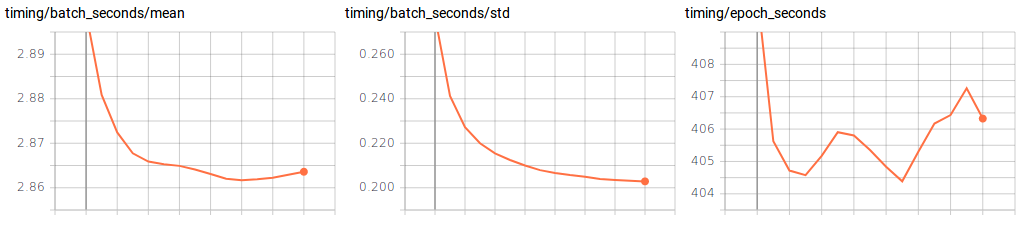
\includegraphics [scale=0.5] {part4/bilstm_timing}
	\caption{Models batch time by epochs} 
	\label{img:bilstm_timing}  
\end{figure}


Histograms give much information about what is happening with the network. I decided to pay attention to histograms which were output from the recurrent network - that show bi-LSTM behavior and weights for first layer of feedforward network. I did not find a descriptive explanation for how to interpret these kinds of graphics, so I followed basic knowledge from statistics. 

\begin{figure}[ht]
	\begin{minipage}[ht]{1\linewidth}
		\center{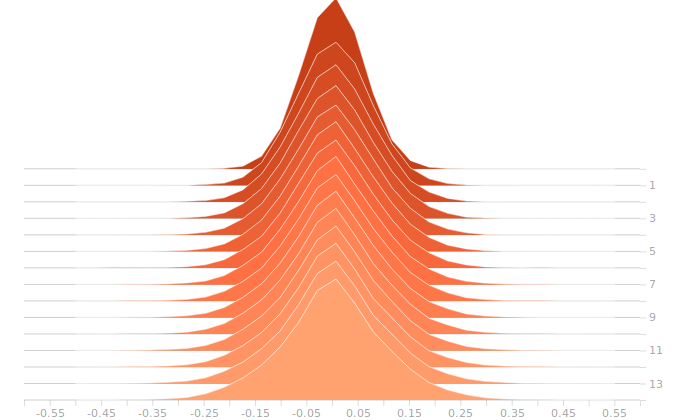
\includegraphics[width=0.5\linewidth]{part4/bilstm_forward_lstm_1_recurrent_kernel_0} \\ а}
	\end{minipage}
	\hfill
	\begin{minipage}[ht]{1\linewidth}
		\center{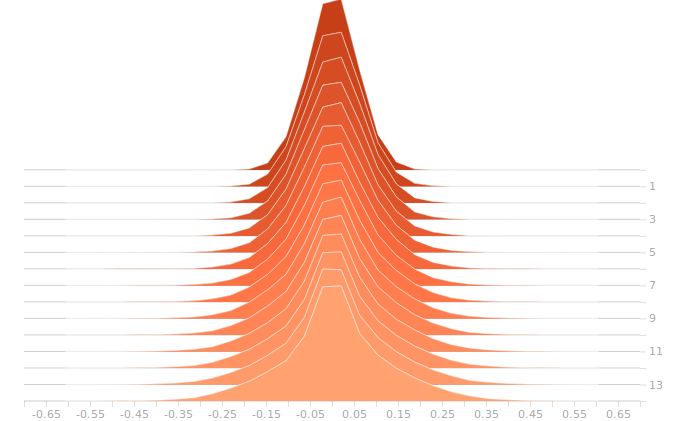
\includegraphics[width=0.5\linewidth]{part4/bilstm_backward_lstm_1_recurrent_kernel_0} \\ b}
	\end{minipage}
	\caption{Bi-LSTM 100 units. Histogram of output from forward recurrent layers (a); histogram of weights from backward recurrent layers (b)}
	\label{img:Bi-LSTM 100 units. Histogram of output from forward recurrent}  
\end{figure}


According to Figures \ref{img:/bilstm_val_category_accuracy}, \ref{img:bilstm_val_category_crossentropy}, \ref{img:bilstm_val_top_k_accuracy} model was not overfitted. Histograms of outputs from feed forward and backward recurrent layers Figure \ref{img:Bi-LSTM 100 units. Histogram of output from forward recurrent} do not change significantly during training process. 
This can be explained by the fact that this layer does not train enough and I think that this network continues to learn thanks to FFNN part Figure \ref{img:bilstm_dense}. I think, that the best shape for the histogram of weights from first FFNN layer will be a normal distribution with higher variance, than after initialization. As we can see the FFNN layer has exactly such behavior which means that it learns some meaningful information. It is possible that more epochs will have a positive effect on the recurrent layer. 

\begin{figure}[ht] 
	\center
	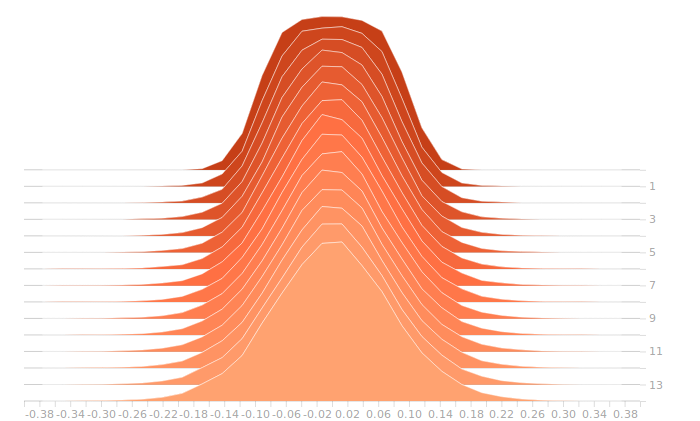
\includegraphics [scale=0.5] {part4/bilstm_dense}
	\caption{Bi-LSTM 100 units. Histogram of weights from first FFNN layer.} 
	\label{img:bilstm_dense}  
\end{figure}

The bi-LSTM model requires a significant amount of computational resources: especially RAM.
Therefore, a batch size was chosen equal to 3048. We can see consumption of resources in Figure \ref{img:resources_BILSTM}


\begin{figure}[ht] 
	\center
	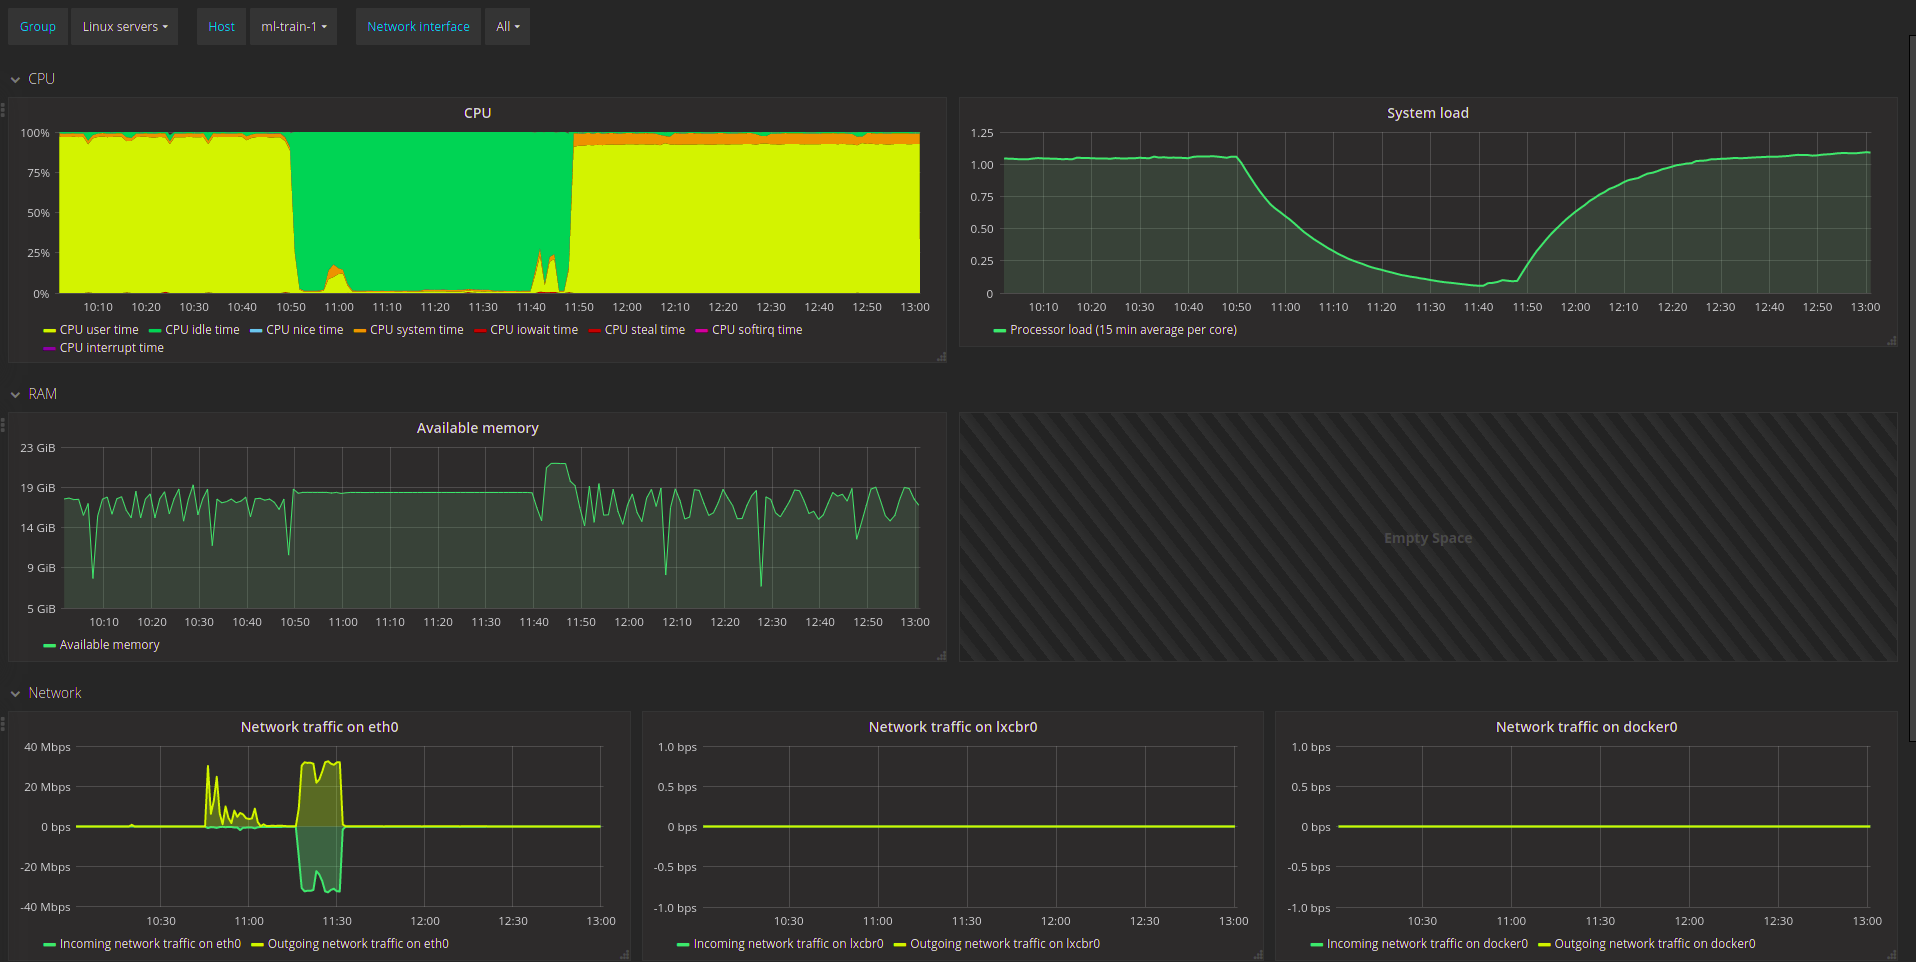
\includegraphics [scale=0.2] {part4/resources_BILSTM}
	\caption{CPU resources which were used while training Bi-LSTM NN.} 
	\label{img:resources_BILSTM}  
\end{figure}


\clearpage
\section{Convolution neural network} \label{sect4_3}

In this part, I would like to show that CNN can perform not worse than recurrent based neural networks. Therefore, I implemented CNN architecture Figure \ref{img:cnn_architecture} which was described in the section \ref{sect2_2_1}. I build three model with different numbers of filters. The smallest one contains 128 filters, middle one - 256 and the biggest - 512. All models were trained with the same number of filter: 3, 4, 5 and dropout rate equals to 0.5. I did not use regularization for convolution layers, but according to my experience, big pooling window also prevent overfitting.Models were trained on 15 epochs.

Let us compare results which different models give. 

\begin{table}[h]
	\centering
	\caption{Analysis of categorical accuracy}
	\label{my-label}
	\begin{tabular}{| p{7cm} | p{3cm} | p{3cm} |}
		%	\begin{tabulary}{1.0\textwidth}{|L|L|L|L|L|L}
		\hline
		\textbf{Number of filters}  & \textbf{Train} & \textbf{Test}                                                    
		\\ \hline
		128   &  0.8165 & 0.8126
		\\ \hline
		256   &  0.8532 & 0.8251 
		\\ \hline
		512   &  0.8885 & 0.8338
		\\ \hline		
	\end{tabular}
\end{table}


\begin{figure}[ht]
	\begin{minipage}[ht]{1\linewidth}
		\center{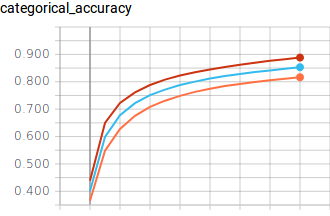
\includegraphics[width=0.5\linewidth]{part4/3CNN_train_category_accuracy}}
	\end{minipage}
	\hfill
	\begin{minipage}[ht]{1\linewidth}
		\center{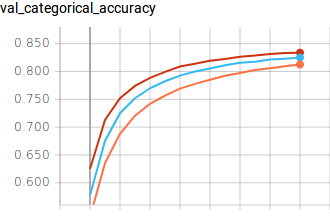
\includegraphics[width=0.5\linewidth]{part4/3CNN_val_category_accuracy}}
	\end{minipage}
	\caption{Models train and validation categorical accuracy by epochs}
	\label{img:3CNN_categorical_accuracy}  
\end{figure}


\begin{table}[h]
	\centering
	\caption{Analysis of category crossentropy}
	\label{my-label}
	\begin{tabular}{| p{7cm} | p{3cm} | p{3cm} |}
		%	\begin{tabulary}{1.0\textwidth}{|L|L|L|L|L|L}
		\hline
		\textbf{Number of filters}  & \textbf{Train} & \textbf{Test}                                                    
		\\ \hline
		128   &  0.8060 & 0.8434
		\\ \hline
		256   &  0.6340 & 0.7746 
		\\ \hline
		512   &  0.4731 & 0.7331
		\\ \hline		
	\end{tabular}
\end{table}

\begin{figure}[ht]
	\begin{minipage}[ht]{1\linewidth}
		\center{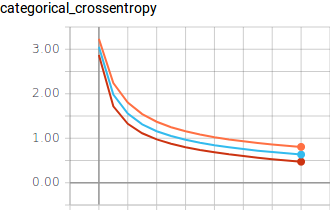
\includegraphics[width=0.5\linewidth]{part4/3CNN_train_category_crossentropy}}
	\end{minipage}
	\hfill
	\begin{minipage}[ht]{1\linewidth}
		\center{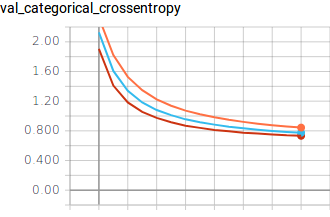
\includegraphics[width=0.5\linewidth]{part4/3CNN_val_category_crossentropy}}
	\end{minipage}
	\caption{Models train and validation category crossentropy by epochs}
	\label{img:3CNN_category_crossentropy}  
\end{figure}


\begin{table}[h]
	\centering
	\caption{Analysis of top k accuracy}
	\label{my-label}
	\begin{tabular}{| p{7cm} | p{3cm} | p{3cm} |}
		%	\begin{tabulary}{1.0\textwidth}{|L|L|L|L|L|L}
		\hline
		\textbf{Number of filters}  & \textbf{Train} & \textbf{Test}                                                    
		\\ \hline
		128   &  0.9259 & 0.9191
		\\ \hline
		256   &  0.9495 & 0.9286 
		\\ \hline
		512   &  0.9696 & 0.9342
		\\ \hline		
	\end{tabular}
\end{table}


According to the results \ref{img:3CNN_categorical_accuracy}, \ref{img:3CNN_category_crossentropy}, \ref{img:3CNN_top_k_accuracy}, \ref{img:3CNN_timing}, I can assume that models having more filters show better accuracy. However, it is noticeable that model with 256 and 512 filters have quite different results on train and test sets (~3-5\% difference). It can be interpreted as overfitting of these models. 


\begin{figure}[ht]
	\begin{minipage}[ht]{1\linewidth}
		\center{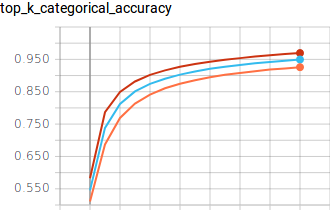
\includegraphics[width=0.5\linewidth]{part4/3CNN_train_top_k_accuracy}}
	\end{minipage}
	\hfill
	\begin{minipage}[ht]{1\linewidth}
		\center{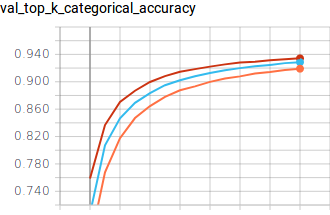
\includegraphics[width=0.5\linewidth]{part4/3CNN_val_top_k_accuracy}}
	\end{minipage}
	\caption{Models train and validation top k accuracy by epochs}
	\label{img:3CNN_top_k_accuracy}  
\end{figure}


\begin{figure}[ht] 
	\center
	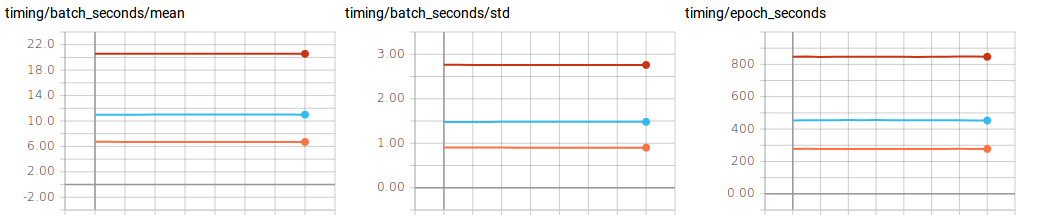
\includegraphics [scale=0.5] {part4/3CNN_timing}
	\caption{Models batch time by epochs} 
	\label{img:3CNN_timing}  
\end{figure}

\clearpage

Histograms of convolution layers Figure \ref{img:3CNN_conv_layers} look almost the same. They do not change significantly from the initial distribution. It can mean these layers do not learn much. 

\begin{figure}[ht]
	\begin{minipage}[ht]{1\linewidth}
		\center{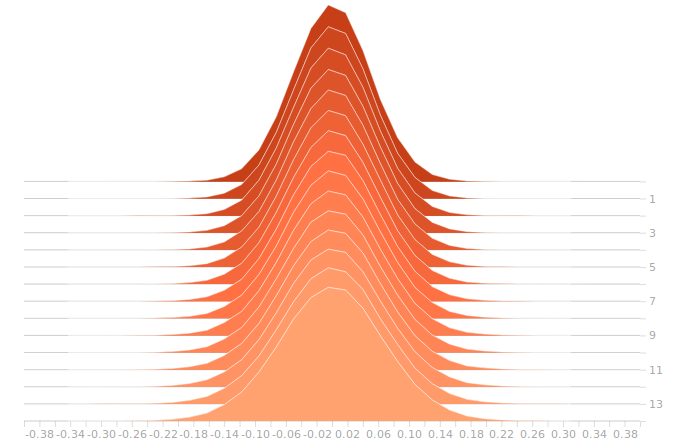
\includegraphics[width=0.5\linewidth]{part4/3CNN-conv-128.png} \\ а}
	\end{minipage}
	\hfill
	\begin{minipage}[ht]{1\linewidth}
		\center{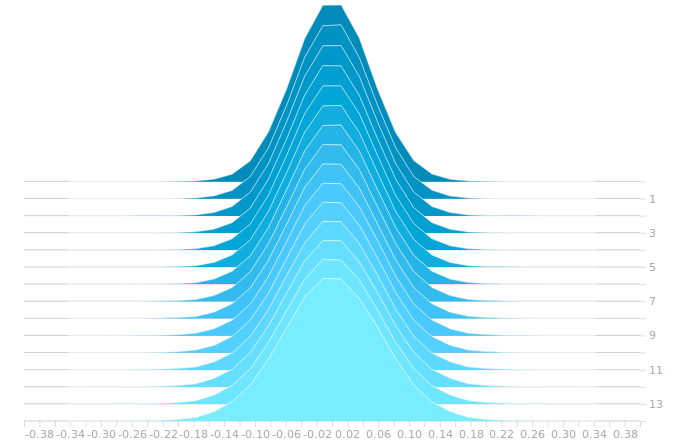
\includegraphics[width=0.5\linewidth]{part4/3CNN-conv-256.png} \\ b}
	\end{minipage}
	\begin{minipage}[ht]{1\linewidth}
		\center{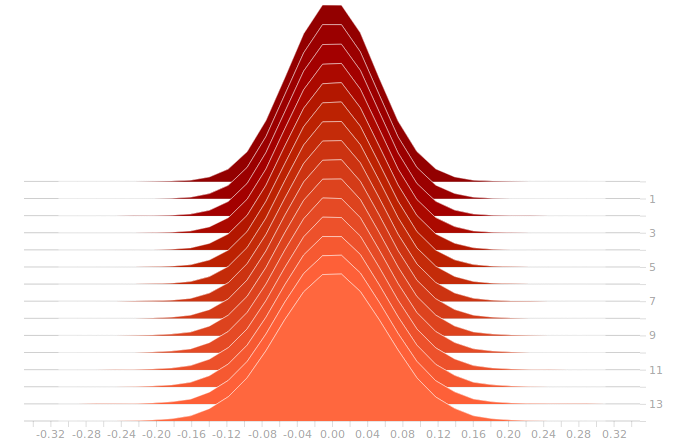
\includegraphics[width=0.5\linewidth]{part4/3CNN-conv-512.png} \\ c}
	\end{minipage}
	\caption{Convolutional model (a) 128;(b) 256; (c) 512 filters for each sizes [3, 4, 5]. Histogram of convolution layers}
	\label{img:3CNN_conv_layers}  
\end{figure}

\noindent
\\
\\
\\
\\
\\
Merged layers Figure \ref{img:3CNN_merged_layers} are also very similar, because of convolution layers.

\begin{figure}[ht]
	\begin{minipage}[ht]{1\linewidth}
		\center{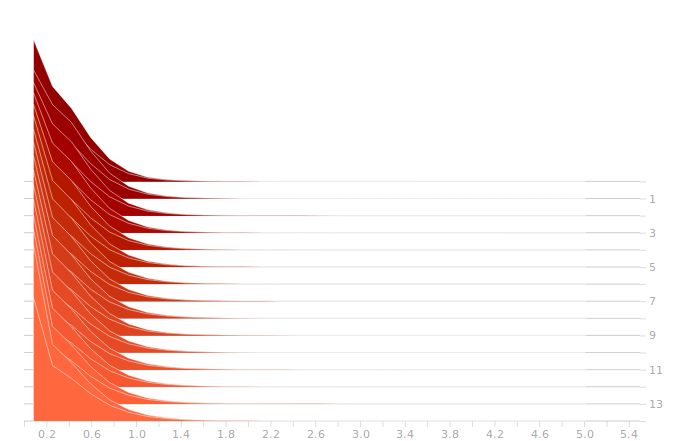
\includegraphics[width=0.45\linewidth]{part4/3CNN-merge3-128.png} \\ а}
	\end{minipage}
	\hfill
	\begin{minipage}[ht]{1\linewidth}
		\center{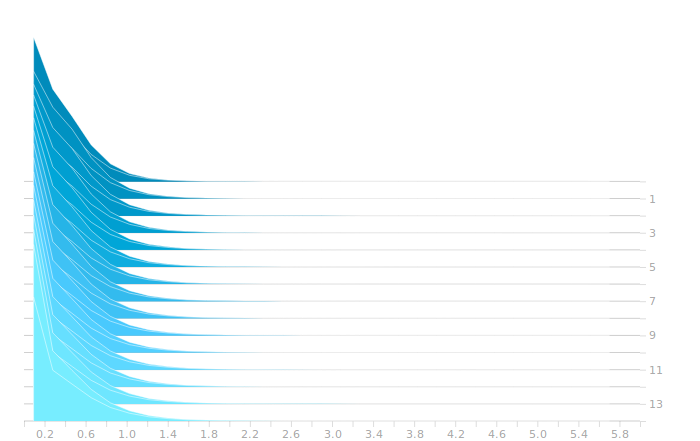
\includegraphics[width=0.45\linewidth]{part4/3CNN-merge3-256.png} \\ b}
	\end{minipage}
	\begin{minipage}[ht]{1\linewidth}
 		\center{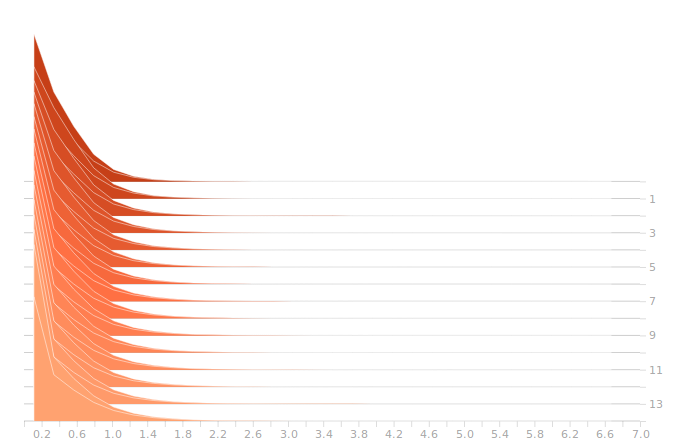
\includegraphics[width=0.45\linewidth]{part4/3CNN-merge3-512.png} \\ c}
	\end{minipage}
	\caption{Convolutional model (a) 128;(b) 256; (c) 512 filters for each sizes [3, 4, 5]. Histogram of merged layers}
	\label{img:3CNN_merged_layers}  
\end{figure}

\clearpage
We can easily notice the difference in the shape of the distribution Figure \ref{img:3CNN_dense_layers} on the initial epoch and the final. The model with 512 filters has a normal distribution with lower variance comparing to the one with 128 filters. It is noticeable, that this the final distribution changed comparing to initial one, that means that layer learned some information. 

\begin{figure}[ht]
	\begin{minipage}[ht]{1\linewidth}
		\center{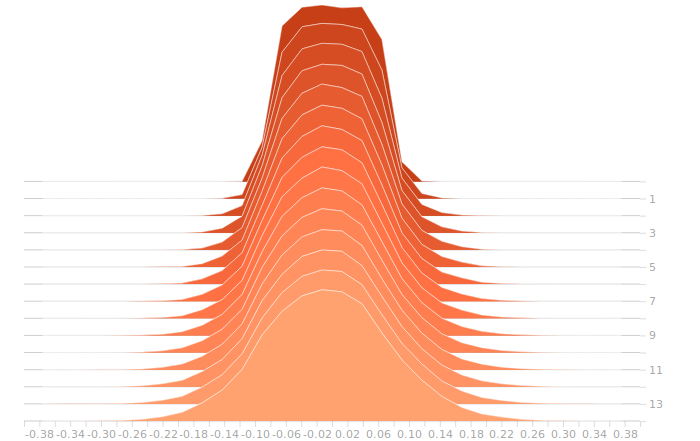
\includegraphics[width=0.5\linewidth]{part4/3CNN-dense-128.png} \\ а}
	\end{minipage}
	\hfill
	\begin{minipage}[ht]{1\linewidth}
		\center{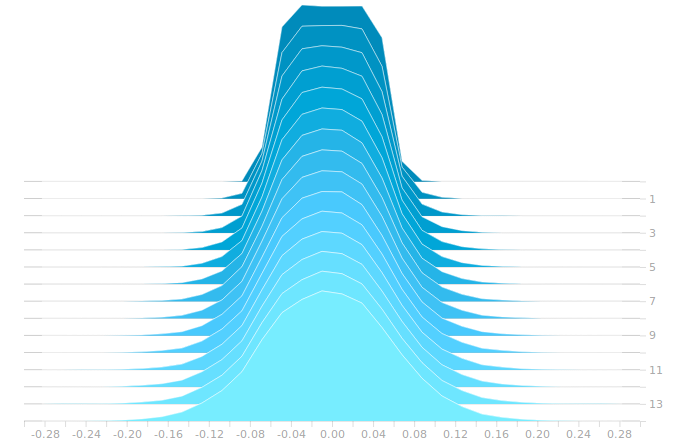
\includegraphics[width=0.5\linewidth]{part4/3CNN-dense-256.png} \\ b}
	\end{minipage}
	\begin{minipage}[ht]{1\linewidth}
		\center{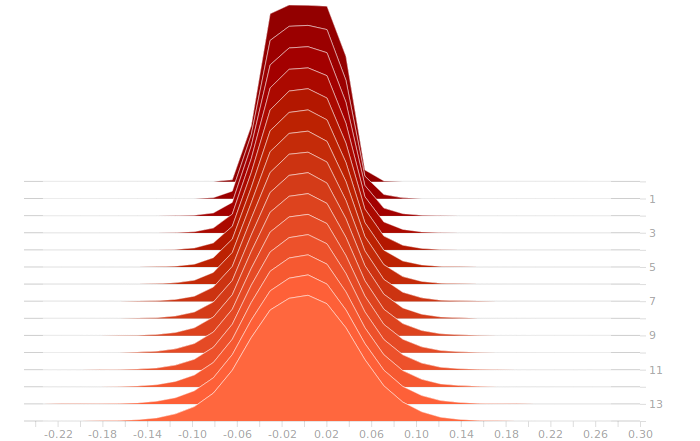
\includegraphics[width=0.5\linewidth]{part4/3CNN-dense-512.png} \\ c}
	\end{minipage}
	\caption{Convolutional model (a) 128;(b) 256; (c) 512 filters for each sizes [3, 4, 5]. Histogram of dense layers}
	\label{img:3CNN_dense_layers}  
\end{figure}

\clearpage
The CNN model requires fewer resources for training than bi-LSTM. Therefore, I was able to use 
5 times bigger batch size. We can see consumption of resources in the Figure \ref{img:resources_CNN}

\begin{figure}[ht] 
	\center
	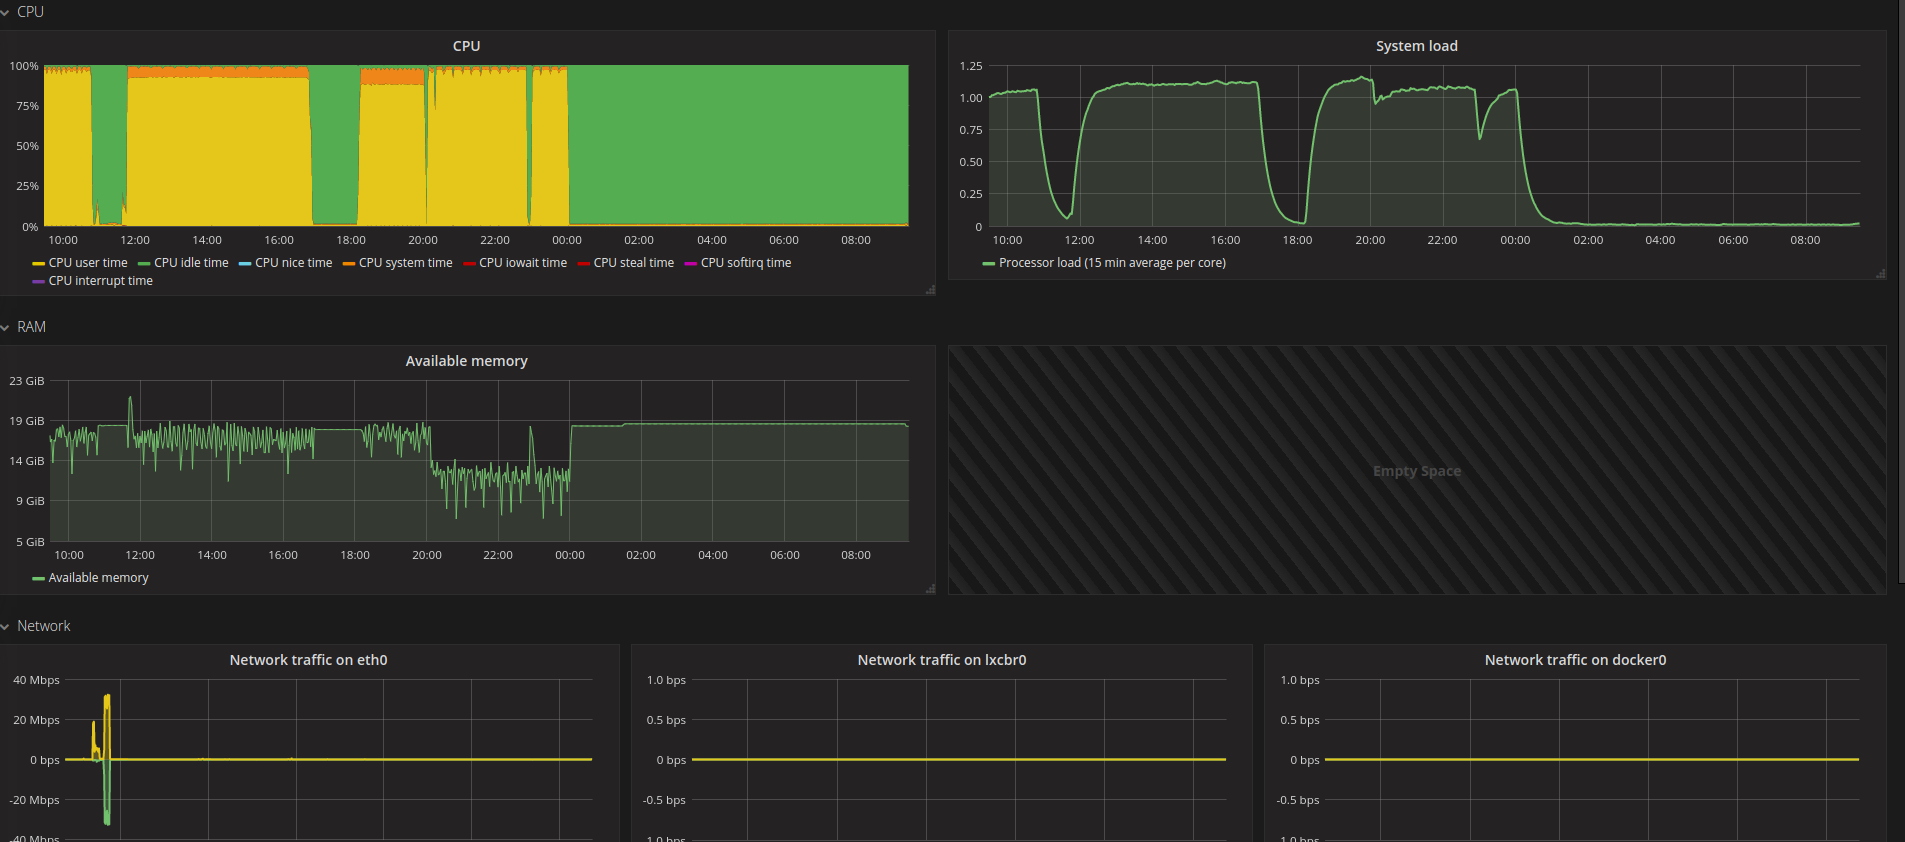
\includegraphics [scale=0.2] {part4/resources_CNN}
	\caption{CPU resources which were used while training CNN.} 
	\label{img:resources_CNN}  
\end{figure}




\clearpage
\section{Convolution neural network with different regularization} \label{sect4_4}

In this section, I tried to use different regularization to get rid of overfitting. I tested all these approaches on the CNN with 512 filters. I made the following changes in the initial architecture of the model:

%blue-modified_epoch15_outdim183_nbfilters512_drop10.5_drop20.2
%grey-withl2regul_0.001_0.01_adam_epoch15_outdim183_nbfilters512_drop10.25_drop20.25
%pink-withl2regul_0.001_0.01_epoch15_outdim183_nbfilters512_drop10.25_drop20.25
%cyan-withl2regul_epoch15_outdim183_nbfilters512_drop10.25_drop20.25


Modifications:
\begin{enumerate}
	\item In the previous section the convolution layer did not train enough,
	 so I thought it was caused because of big dropout rate. Therefore I decreased it in two times.
	\item I also added the l2-regularization equals to 0.01 both for convolution layers and dense layer. 
	Dropout equals to the rate 0.5 both for dense and convolution layers. 
	Moreover, I decided to configure my training algorithm, so I used Adam with learning rate 1e-4. 
	\item l2-regularization equals to 0.001 for convolution layers and 0.01 for dense layer. 
	Adam was with learning rate 1e-3. 
	Dropout rate equals to 0.25 both for dense and convolution layers. 
	\item l2-regularization equals to 0.001 for convolution layers and 0.01 for dense layers. 
	Dropout rate equals to 0.25 for convolution layers and 0.5 for dense layers.
\end{enumerate}

\begin{table}[h]
	\centering
	\caption{Analysis of categorical accuracy}
	\label{my-label}
	\begin{tabular}{| p{3cm} | p{3cm} | p{3cm} |}
		%	\begin{tabulary}{1.0\textwidth}{|L|L|L|L|L|L}
		\hline
		\textbf{Modification type}  & \textbf{Train} & \textbf{Test}                                                    
		\\ \hline
		1   &  0.8321 & 0.7993
		\\ \hline
		2   &  0.7101 & 0.7146 
		\\ \hline
		3   &  0.9026 & 0.7882
		\\ \hline		
		4   &  0.8514 & 0.7449
		\\ \hline
	\end{tabular}
\end{table}

\begin{table}[h]
	\centering
	\caption{Analysis of categorical cross entropy}
	\label{my-label}
	\begin{tabular}{| p{3cm} | p{3cm} | p{3cm} |}
		%	\begin{tabulary}{1.0\textwidth}{|L|L|L|L|L|L}
		\hline
		\textbf{Modification type}  & \textbf{Train} & \textbf{Test}                                                    
		\\ \hline
		1   &  0.7894 & 0.9405
		\\ \hline
		2   &   1.504 &  1.7040
		\\ \hline
		3   &  0.4928 & 1.4280
		\\ \hline		
		4   &  0.7151 & 1.6890
		\\ \hline
	\end{tabular}
\end{table}

\begin{table}[h]
	\centering
	\caption{Analysis of top k accuracy}
	\label{my-label}
	\begin{tabular}{| p{3cm} | p{3cm} | p{3cm} |}
		%	\begin{tabulary}{1.0\textwidth}{|L|L|L|L|L|L}
		\hline
		\textbf{Modification type}  & \textbf{Train} & \textbf{Test}                                                    
		\\ \hline
		1   &  0.9681 & 0.9348
		\\ \hline
		2  &   0.8333 & 0.8363
		\\ \hline
		3   &  0.9704 & 0.9179
		\\ \hline		
		4   &  0.9453 & 0.8921
		\\ \hline
	\end{tabular}
\end{table}

\noindent
\\
According to the results Figures \ref{img:4CNN_categorical_accuracy}, \ref{img:4CNN_category_crossentropy}, \ref{img:4CNN_top_k_accuracy}, \ref{img:4CNN_timing}, it can be clearly seen that model with modifications number 3 and 4 were overfitted for sure.
Model number 1 has lower overfit rate. The most stable model was number 2, which demonstrated the same results on test and train dataset. 

\begin{figure}[ht]
	\begin{minipage}[ht]{1\linewidth}
		\center{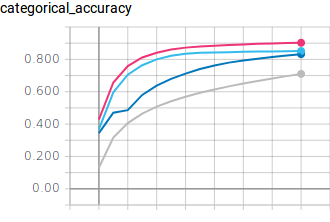
\includegraphics[width=0.5\linewidth]{part4/4CNN_train_category_accuracy}}
	\end{minipage}
	\hfill
	\begin{minipage}[ht]{1\linewidth}
		\center{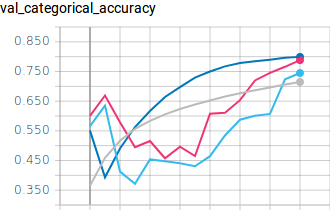
\includegraphics[width=0.5\linewidth]{part4/4CNN_val_category_accuracy}}
	\end{minipage}
	\caption{Models train and validation categorical accuracy by epochs}
	\label{img:4CNN_categorical_accuracy}  
\end{figure}


\begin{figure}[ht]
	\begin{minipage}[ht]{1\linewidth}
		\center{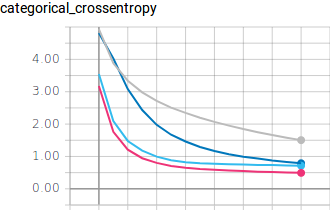
\includegraphics[width=0.5\linewidth]{part4/4CNN_train_category_crossentropy}}
	\end{minipage}
	\hfill
	\begin{minipage}[ht]{1\linewidth}
		\center{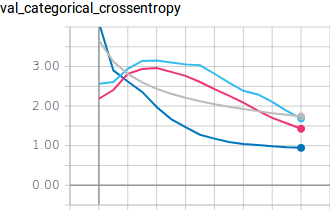
\includegraphics[width=0.5\linewidth]{part4/4CNN_val_category_crossentropy}}
	\end{minipage}
	\caption{Models train and validation category crossentropy by epochs}
	\label{img:4CNN_category_crossentropy}  
\end{figure}

\begin{figure}[ht]
	\begin{minipage}[ht]{1\linewidth}
		\center{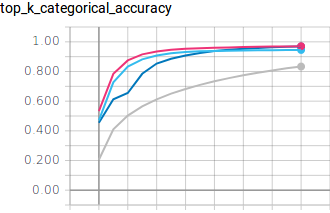
\includegraphics[width=0.5\linewidth]{part4/4CNN_train_top_k_accuracy}}
	\end{minipage}
	\hfill
	\begin{minipage}[ht]{1\linewidth}
		\center{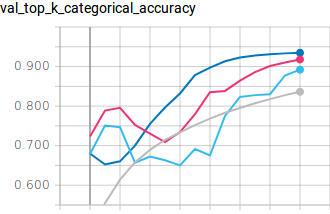
\includegraphics[width=0.5\linewidth]{part4/4CNN_val_top_k_accuracy}}
	\end{minipage}
	\caption{Models train and validation top k accuracy by epochs}
	\label{img:4CNN_top_k_accuracy}  
\end{figure}

\begin{figure}[ht] 
	\center
	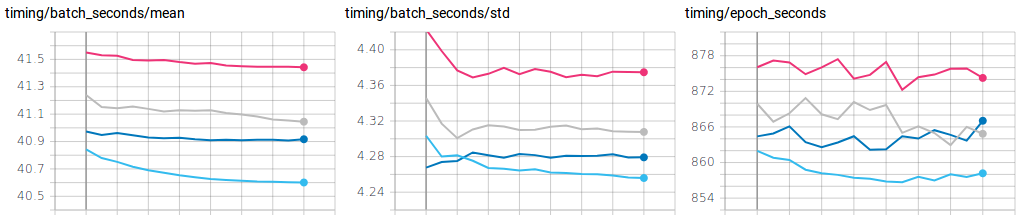
\includegraphics [scale=0.5] {part4/4CNN_timing}
	\caption{Models batch time by epochs} 
	\label{img:4CNN_timing}  
\end{figure}

 
\begin{figure}[ht]
	\begin{minipage}[ht]{1\linewidth}
		\center{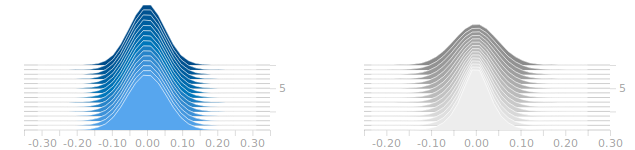
\includegraphics[width=1\linewidth]{part4/4CNN-conv-1.png} \\ а, b}
	\end{minipage}
	\hfill
	\begin{minipage}[ht]{1\linewidth}
		\center{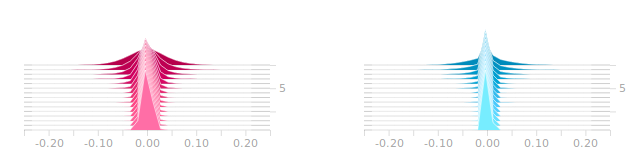
\includegraphics[width=1\linewidth]{part4/4CNN-conv-2.png} \\ c, d}
	\end{minipage}
	\caption{Convolutional models with modification (a) 1;(b) 2; (c) 3; (d) 4. Histogram of convolution layers}
	\label{img:Convolutional models with modification convolution layers}  
\end{figure}

\clearpage
If we compare results of weights histograms Figures \ref{img:Convolutional models with modification convolution layers}, \ref{img:Convolutional models with modification merged layers} with the ones in Section \ref{sect4_3} we can see a significant difference in distributions.
Which is mostly caused by different types of regularizations. We can also see that convolution layers from model 1 and 3 change through epochs which
means that they learn.  

\begin{figure}[ht]
	\begin{minipage}[ht]{1\linewidth}
		\center{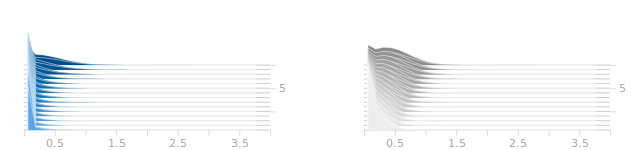
\includegraphics[width=1\linewidth]{part4/4CNN-merge3-1.png} \\ а, b}
	\end{minipage}
	\hfill
	\begin{minipage}[ht]{1\linewidth}
		\center{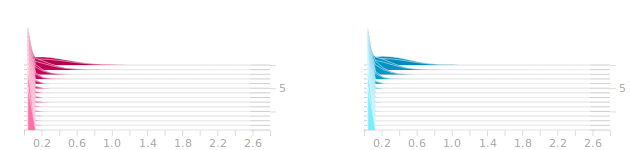
\includegraphics[width=1\linewidth]{part4/4CNN-merge3-2.png} \\ c, d}
	\end{minipage}
	\caption{Convolutional models with modification (a) 1;(b) 2; (c) 3; (d) 4. Histogram of merged layers}
	\label{img:Convolutional models with modification merged layers}  
\end{figure}

\clearpage
Similar situation we can see with dense layers Figure \ref{img:Convolutional models with modification Histogram of dense layers}. The weights are put into ranges between -0.1 and 0.1 where l2-regularizations was used.
The changes through epochs we can see only in first two models which are marked with blue and gray colors.   

\begin{figure}[ht]
	\begin{minipage}[ht]{1\linewidth}
		\center{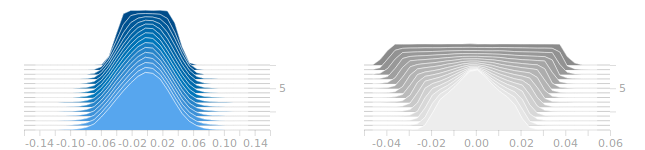
\includegraphics[width=1\linewidth]{part4/4CNN-dense-1.png} \\ а, b}
	\end{minipage}
	\hfill
	\begin{minipage}[ht]{1\linewidth}
		\center{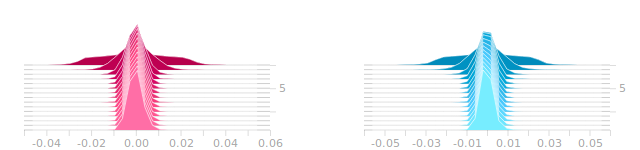
\includegraphics[width=1\linewidth]{part4/4CNN-dense-2.png} \\ c, d}
	\end{minipage}
	\caption{Convolutional models with modification (a) 1;(b) 2; (c) 3; (d) 4.  Histogram of dense layers}
	\label{img:Convolutional models with modification Histogram of dense layers}  
\end{figure}


As we can see regularizations play the key role to avoid overfitting of the models. High dropout rate in combination with l2-regularization for dense and convolutions layers showed the best stability. Therefore, I chose model number 2 for the further training. 

\clearpage
\section{Final model} \label{sect4_5}

In this section I trained the best model from the Section \ref{sect4_5} on 25 epochs.
I has following parameters:

\begin{itemize}
	\item 300 filters
	\item size of filter: 3, 4, 5
	\item l2-regularization equals to 0.01 both for convolution layers and dense layer. 
	\item dropout equals to the rate 0.5 both for dense and convolution layers. 
	\item learning algorithm Adam with learning rate 1e-4. 
\end{itemize}

One more modification which was made: from the previous Section \ref{sect4_5}
according to many metrics model with these configurations trained slower than others because 
it has the lowest learning rate 1e-4. To speed up the training process I increased the learning rate in the beginning to be equal 1e-3. Then as the CNN slowly converges to its optimal value
the learning was decreased to 1e-4 to slow down - otherwise it may overshoot the optimal value.
Such modifications gave me improvement in speed and the stability of the model at the same time.
The final results can be seen in Figures \ref{img:final_CNN_categorical_accuracy}, 
\ref{img:final_CNN_category_crossentropy}, \ref{img:final_CNN_top_k_accuracy}.


\begin{table}[h]
	\centering
	\caption{Final results}
	\label{my-label}
	\begin{tabular}{| p{7cm} | p{3cm} | p{3cm} |}
		%	\begin{tabulary}{1.0\textwidth}{|L|L|L|L|L|L}
		\hline
		\textbf{Metric}  & \textbf{Train} & \textbf{Test}                                                    
		\\ \hline
		categorical accuracy   &  0.8250 & 0.8307
		\\ \hline
		category crossentropy  &   0.5800 & 0.6612
		\\ \hline
		top k accuracy   &  0.9545 & 0.9473
		\\ \hline		
	\end{tabular}
\end{table}

	


\begin{figure}[ht]
	\begin{minipage}[ht]{1\linewidth}
		\center{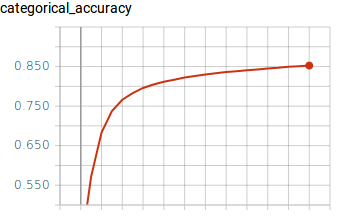
\includegraphics[width=0.5\linewidth]{part4/final_CNN_train_category_accuracy}}
	\end{minipage}
	\hfill
	\begin{minipage}[ht]{1\linewidth}
		\center{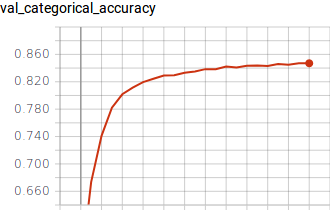
\includegraphics[width=0.5\linewidth]{part4/final_CNN_val_category_accuracy}}
	\end{minipage}
	\caption{Models train and validation categorical accuracy by epochs}
	\label{img:final_CNN_categorical_accuracy}  
\end{figure}


\begin{figure}[ht]
	\begin{minipage}[ht]{1\linewidth}
		\center{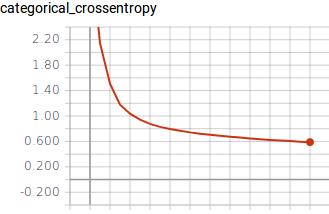
\includegraphics[width=0.5\linewidth]{part4/final_CNN_train_category_crossentropy}}
	\end{minipage}
	\hfill
	\begin{minipage}[ht]{1\linewidth}
		\center{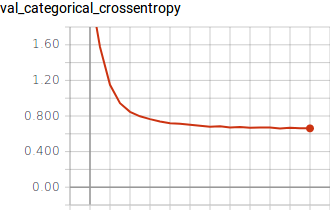
\includegraphics[width=0.5\linewidth]{part4/final_CNN_val_category_crossentropy}}
	\end{minipage}
	\caption{Models train and validation category crossentropy by epochs}
	\label{img:final_CNN_category_crossentropy}  
\end{figure}

\clearpage
\begin{figure}[ht]
	\begin{minipage}[ht]{1\linewidth}
		\center{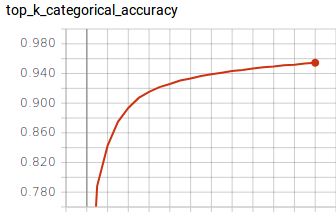
\includegraphics[width=0.5\linewidth]{part4/final_CNN_train_top_k_accuracy}}
	\end{minipage}
	\hfill
	\begin{minipage}[ht]{1\linewidth}
		\center{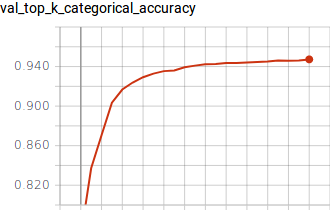
\includegraphics[width=0.5\linewidth]{part4/final_CNN_val_top_k_accuracy}}
	\end{minipage}
	\caption{Models train and validation top k accuracy by epochs}
	\label{img:final_CNN_top_k_accuracy}  
\end{figure}


\begin{longtable}[c]{|l|c|c|l|l|}
	\caption[Classification report]{Classification report}
	\label{tab:amortecimentos_1}\\
	\hline  category & precision & recall &  f1-score & support\\ \hline
	\endhead
	\hline
	\endlastfoot
	
	1        & 0         & 0      & 0        & 7       \\
	3        & 0         & 0      & 0        & 4       \\
	4        & 0         & 0      & 0        & 2       \\
	11       & 0.78      & 0.58   & 0.66     & 623     \\
	14       & 0.93      & 0.99   & 0.96     & 8070    \\
	15       & 0.82      & 0.68   & 0.74     & 362     \\
	16       & 0.93      & 0.95   & 0.94     & 1656    \\
	20       & 0.82      & 0.91   & 0.86     & 1151    \\
	25       & 0.75      & 0.9    & 0.82     & 1910    \\
	29       & 0.97      & 0.99   & 0.98     & 12346   \\
\end{longtable}

Here is the concise version of final classification report for each class. Full version can be found in APPENDIX B. As we can see in the Table \ref{amortecimentos_1} model showed the best results on the categories with big number of advertisements: 14, 29. It makes mistakes on categories with less samples: 11 and 15 respectively and can hardly ever make a right predictions on the categories where the number of observations are less then 10. 

\section{Summary of the section} \label{sect4_6}

In this section I have made a series of
experiments with recurrent and convolutional neural networks
built on top of word2vec. I did a little tuning
of hyperparameters to achieve the highest scores. 
According to the results of experiments which CNN models achieved, are the same and in some components even better than the ones of Bi-LSTM models.I can make a conclusion that Convolution Neural Networks perform remarkably well for NLP related problems and specially for text classification. 


